\documentclass[12pt,a4paper,oneside,openright]{report}

\usepackage[utf8]{inputenc}
\usepackage[italian]{babel}
\usepackage[T1]{fontenc}
\usepackage{latexsym}
\usepackage{graphicx}
\usepackage{epsfig}
\usepackage{amsmath,amssymb,amsthm}
\usepackage[none]{hyphenat} 
\usepackage{float} % parametro H in figur : posizionamento esattamente li
\usepackage{verbatim}
\usepackage{booktabs}
\usepackage{enumerate} %lettere o altro negli indici
\usepackage{algorithmic} %float con un algoritmo
\usepackage[boxed]{algorithm}
\usepackage{subfig}    % + figure in un float figure

%con la classe book+openright lascio una pagina bianca a fine capitolo e dopo il titolo se necessario, con empty page queste pagine non sono numerate e non hanno stile
%%\usepackage{emptypage}



\usepackage{fancyhdr}
\setcounter{tocdepth}{3}

\makeatletter

% 1 freccia andata ritorno per scriverci sopra
\newcommand{\xleftrightarrow}[2][]{%
  \ext@arrow3399{\longleftrightarrowfill@}{#1}{#2}}
\newcommand{\longleftrightarrowfill@}{%
  \arrowfill@\leftarrow\relbar\rightarrow}

% 2 frecce andata ritorno per scriverci sopra
\def\rightharpoonupfill@{%
  \arrowfill@\relbar\relbar\rightharpoonup}
\def\leftharpoondownfill@{%
  \arrowfill@\leftharpoondown\relbar\relbar}


\newcommand{\xrightleftharpoons}[2][]{\mathrel{%
\raise.22ex\hbox{%
$\ext@arrow 3095\rightharpoonupfill@{\phantom{#1}}{#2}$}%
\setbox0=\hbox{%
$\ext@arrow 0359\leftharpoondownfill@{#1}{\phantom{#2}}$}%
\kern-\wd0 \lower.22ex\box0}%
}

\renewcommand{\algorithmicrequire}{\textbf{Input:}}
\renewcommand{\algorithmicensure}{\textbf{Output:}}

\makeatother 
\frenchspacing
%\pagestyle{headings} % {headings,plain ,empty}
\linespread{1.3}
\DeclareGraphicsRule{.eps,.ps,.png}{bmp}{.bb}{} % formati utilizzabili con ordine di preferenza 
                                                % cosi non devo indicare le estensioni
\newcommand{\HRule}{\rule{\linewidth}{0.5mm}}


%\author{\emph{Marco Bettiol}\quad{} 586580\\\emph{Antonio Quercia}\quad{}  588537}

%per impaginare con giustifica sx-dx
  \tolerance 1414
  \hbadness 1414
  \emergencystretch 1.5em
  \hfuzz 0.3pt
  \widowpenalty=10000
  \vfuzz \hfuzz
  \raggedbottom

\title{}
\begin{document}
% !TEX root = tesi.tex
\begin{titlepage}

		\thispagestyle{empty}
    \begin{figure}
    \centering
      \subfloat{
\includegraphics[scale=1]{immagini/logo_unipd_black}}\quad     \subfloat{
\includegraphics[scale=1.3]{immagini/DEIlogoFULL}}
    \end{figure}
    
    \vskip 3cm{
    \begin{center}\sc
        UNIVERSITY OF PADUA\\
        DEPARTMENT OF INFORMATION ENGINEERING\\
        MASTER DEGREE IN COMPUTER ENGINEERING\end{center}
		}
		
		\vskip1.2cm\begin{center}
      \rm\large\uppercase\expandafter{A.A. 2009/2010\\}
 \end{center}
    	
    \vskip 2.5cm\begin{center}
    \HRule \\[0.4cm]\LARGE\expandafter{BATCH SIZE ESTIMATE}
    \HRule \\[0.4cm]
    \end{center}
    
    \begin{flushright}\vskip4.0cm 
    \begin{tabular}{rl}
            \rm\large \uppercase{Supervisor:} &\emph{Prof. Andrea Zanella}\\
	   \rm\large \uppercase{Student:} &\emph{Marco Bettiol} \\
		\end{tabular}
     \end{flushright}
    \vfill
          \begin{center}
                  \vskip1.0cm 
                  Last Update: \today  \hspace{1mm } \currenttime
           \end{center}
    
\end{titlepage}

\newpage
%%pagina vuota
%\clearpage\null\thispagestyle{empty}\clearpage

%\setcounter{page}{1}

\section*{Introduzione}
Un vettore $x$ di lunghezza N può essere visto come una sequenza $x_0,...,x_{N-1}$ di N numeri complessi. Si definisce $X$ \emph{trasformata discreta di Fourier (DFT, discrete Fourier transform)}  di $x$ la sequenza $X_0,...,X_{N-1}$ espressa dalla seguente relazione:
\begin{equation*}
\label{eq:def-dft}
X_k=\sum_{n=0}^{N-1}x_ne^{-\jmath\frac{2\pi}{N}kn} \quad k=0,...,N-1
\end{equation*}
La \emph{FFT} o \emph{trasformata veloce di Fourier} individua una famiglia di algoritmi in grado di calcolare la DFT in tempo $O(N \log N)$ al posto dell'usuale $O(N^{2})$ ottenibile banalmente attraverso la definizione.\\
Molti di questi algoritmi, oltre che ad essere computazionalmente efficienti, si prestano bene anche ad un'implementazione parallela.\\
In questo lavoro e stata realizzata un'implementazione del noto algoritmo di Cooley-Tukey.
\subsection*{Note su FFT Sequenziale e Cache}
Durante l'implementazione dell'algoritmo è emersa la critica dipendenza tra le prestazioni ottenute dall'algoritmo FFT-DIT2 rispetto alla dimensione della cache della macchina su cui viene lanciato.\\
L'algoritmo implementato infatti, per la natura stessa degli operatori \emph{butterfly}, risulta assolutamente non-cachefriendly.\\
L'accesso in memoria non è locale: ad ogni stadio dell'algoritmo un valore dell'input viene letto/sovrascritto una ed una sola volta. Quando l'accesso ai dati non è spazialmente localizzato e la struttura di computazione è rigida la classica modalità di mapping\\
\begin{center}
\emph{cache address} $=$ \emph{memory address} modulo \emph{cache\_size} 
\end{center}
perde di efficacia. Nel nostro caso si verifica quando la distanza tra i dati da elaborare (potenza di due) è vicina alla dimensione della cache (anch'essa potenza di due).\\
Proponiamo qui di seguito i grafici sullo Cache Miss e MFlops per illustrare la drammaticità del problema.\\
In entrambi i casi le performance diminuiscono drasticamente quando la taglia del problema supera $2^{16}=65536$ per mantenersi successivamente costanti.\\ La diminuzione praticamente lineare delle performance per $N=16$ visibile in Figura \ref{Miss} è conseguenza raddoppio del numero di \emph{twiddle factor} utilizzati ad ogni passo.\\
Le performance inferiori, a parità di stage, per le istanze di taglia maggiore sono probabilmente dovute allo swap in/out dei twiddle factor il cui address mapping entra in conflitto con quello dei valori nel vettore da elaborare.\\
Una volta oltrepassata la soglia critica il Load per Miss si stabilizza sui $5,92$ più di $100$ volte peggiore rispetto agli stage in-cache. 
Analogamente per gli stage out-of-cache si hanno circa $81/60$ Mflops/s.

\begin{figure}[h!]
  \centering
      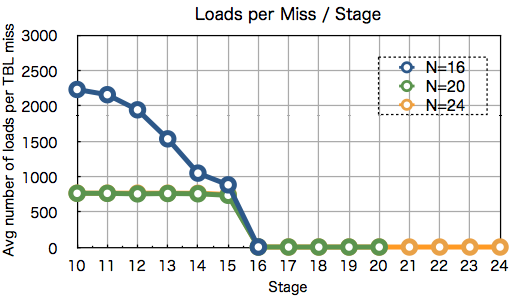
\includegraphics[width=\textwidth]{immagini/Miss}
  \caption{Caricamento di dati utili nei registri / accessi in ram. Maggiore è migliore}
\label{Miss}
\end{figure}

\begin{figure}[h!]
  
  \centering
      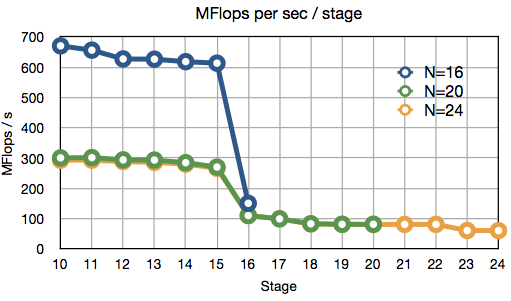
\includegraphics[width=\textwidth]{immagini/Mflops}
  \caption{Potenza di calcolo sfruttata. Maggiore è migliore}
\label{MFlops}
\end{figure}
Notiamo come $N=20$ e $N=24$ abbiano esattamente lo stesso andamento.
\end{document}